\section{Umsetzung}
In diesem Kapitel wird die Vorgehensweise der zuvor beschriebenen Problemstellungen erörtert.

\subsection{Aufbau der Testumgebung}




\subsubsection{Aufsetzen eines Nagios-Test-Systems}
Da die einzelnen Überwachungselemente in der Überwachungssoftware Nagios nach und nach eingetragen (/ definiert / assoziiert / verbunden) werden müssen, ist ein häufiges Neustarten der Nagios Anwendung notwendig, damit die neuen Konfigurationsdateien übernommen werden.

Damit dies nicht auf dem produktiven Nagios-Server durchgeführt werden muss, wird ein Nagios-Testserver für diesen Zwecks eingesetzt.

\subsubsection{Bilddatenbank als VM}
Für die Simulation der verschiedenen Fehlerzuständen der einzelnen Überwachungselemente wird eine virtuelle Maschine mit einer \gls{OracleUCM} Prototypinstallation, die extra als Entwicklungsplattform erstellt wurde, verwendet.


\subsection{Marktübersicht Nagios-Agenten}
Im vorherigen Kapitel \ref{methoden} wurde erklärt, dass für das Überwachen von Diensten, die nicht über das Netzwerk zugreifbar sind, ein Agent auf dem jeweiligen Rechner benötigt wird.

In diesem Unterkapitel werden die populärsten Agenten für Unix und Windows Betriebsysteme aufgelistet und nach/in den Punkten Sicherheit, subjektiver Aufwand für die Konfiguration und Art der Abfragemethode (aktiv oder passiv) vergleicht.
\newpage
\subsubsection{Unix-Agenten}
Für die auf Unix basierenden Betriebsysteme werden fünf verschiedene Möglichkeiten angeboten, die (auch) zuvor in der Abbildung \ref{nagios-kern} als verschiedene Überwachungsmöglichkeiten von Nagios aufgelistet wurden.

%Tabelle Unix-Agenten


\begin{table}[h!]
\centering
\begin{threeparttable}[ht]
\begin{tabular}{l p{1.5cm} l p{1.5cm} l p{1.5cm} l p{1.5cm} l p{1.5cm} l p{1.5cm} p{1.5cm} p{1.5cm} p{1.5cm} p{1.5cm}}
 & \begin{turn}{50}\textbf{SSH}\end{turn} & \begin{turn}{50}\textbf{NRPE}\end{turn} & \begin{turn}{50}\textbf{SNMP}\end{turn} & \begin{turn}{50}\textbf{SNMP Traps}\end{turn} & \begin{turn}{50}\textbf{NSCA}\end{turn}\\ 
\hline
\textbf{Methode} & & & & & \\
\textit{aktiv} & \checkmark & \checkmark & \checkmark & - & - \\
\textit{passiv} & - & - & - & \checkmark & \checkmark\\
\textbf{Sicherheit} &  &  &  &  &  \\
\textit{Passwort} & - & - & \checkmark (v3) & \checkmark (v3) & -\\
\textit{Accesslist}\tnote{*} & \checkmark &  \checkmark & \checkmark (v2) & \checkmark (v2) & \checkmark \\
\textit{Verschlüsselung} &  \checkmark & \checkmark & \checkmark (v3) & \checkmark (v3) &  \checkmark \\
\textbf{Aufwand}\tnote{**} & \begin{footnotesize}leicht\end{footnotesize} & \begin{footnotesize}normal\end{footnotesize} & \begin{footnotesize}hoch\end{footnotesize} & \begin{footnotesize}hoch\end{footnotesize} & \begin{footnotesize}normal\end{footnotesize} \\
\end{tabular}
%\footnotesize
%* Einschränkung der Abfrage der Überwachungsinformationen anhand der \gls{IP}-Adresse
%\\
%** Subjektive Einschätzung
\begin{tablenotes}\footnotesize
      \item[*] Einschränkung der Abfrage der Überwachungsinformationen anhand der \gls{IP}-Adresse
        \item[**] Subjektive Einschätzung
    \end{tablenotes}
\caption{Übersicht der verschiedenen Unix-Agenten}
\end{threeparttable}
\end{table}




Dabei werden drei Agenten genannt, die eine aktive Ausführung der Nagios-Plugins benutzten.
Alle drei Agenten unterscheiden sich jedoch in den (anderen) Punkten Sicherheit und Aufwand.
Der auf \gls{SSH} basierende Agent besitzt einen relativ geringen Aufwand für die Installation, da für den Aufbau der Kommunikation zwischen Nagios-Server und Client nur der öffentliche Schlüssel des Servers auf dem Client eingetragen werden muss.
Dadurch kann der Nagios-Server sich ohne Passwortabfrage an dem zu überwachendem Host anmelden und die sich darauf befindlichen Nagios-Plugins ausführen.
Da auf den meisten Unixservern bereits ein \gls{SSH}-Server läuft und deshalb kein weiterer Port geöffnet oder eine weitere Software installiert werden muss, ist diese Methode den anderen meist vorzuziehen.

Bei der \gls{NRPE}-Methode wird eine weitere Softwarekomponente auf dem Client installiert, die einen separaten Port für die Kommunikation mit dem Nagios-Server öffnet.
Wie bei dem Aufruf per \gls{SSH} müssen sich hier die Nagios-Plugins bereits auf dem Rechner befinden.
Dabei gilt als Unterschied dieser zwei ähnlichen Methoden zu beachten, dass für die Ausführung der Checks per \gls{SSH} ein extra Benutzerkonto auf dem Client erstellt werden muss und somit beliebige Systembefehle ausgeführt werden können, während die Ausführung von Kommandos bei \gls{NRPE} nur auf vorkonfigurierte Befehle beschränkt ist.
Siehe auch Kapitel \ref{sshnrpe}.

Da \gls{SNMP} plattformunabhängig funktioniert ist es mögliche diese Variante bei Unix- sowie bei Windowsservern einzusetzten.
Die verwendete \gls{SNMP}-Version bestimmt welche Sicherheitsmerkmale zur Verfügung stehen.
Zwar gibt es bereits seit Version 1 die Möglichkeit den Zugriff per Passwort in drei Gruppen aufzuteilen: kein Zugriff, Leserecht und Lese- mit Schreibrecht\footnote{Quelle: \cite{Barth08} S. 237}, jedoch wird dieses Passwort im Klartext übertragen, so dass es leicht auslesbar ist.
Auch noch die Version 2 inklusive der erweiterten Version 2c verwendet die gleiche unsichere Authentifizierung.
Erst ab Version 3 wird das Passwort verschlüsselt übertragen.
Während Barth behauptet, dass man bei \gls{SNMP} generell kein Passwort verwenden soll\footnote{Quelle: \cite{Barth08} S. 238}, da es leicht per Netzwerkmitschnittprogramme wie WireShark ausgelesen werden kann, wird in \cite{Jose07} S. 121} klargestellt, dass die Version 3 eine verschlüsselte Authentifizierung durch den MD5- oder SHA-Algorithmus ermöglicht.
Die passive Variante über \gls{SNMP} bei der der Client die Ergebnisse der Checks an den Nagios-Server sendet, auch \gls{SNMP}-Traps genannt, funktioniert nach dem gleichen Prinzip.
Da das Auslesen der \gls{MIB} per SNMP im Gegensatz zu den anderen Varianten deutlich komplexer ist, wird der Aufwand als hoch eingestuft.

Der andere Vertreter, der passive Checks ermöglicht, ist der \gls{NSCA}-Agent.
Wie die anderen Unix-Agenten bietet es die Möglichkeit den Datenaustausch zwischen Nagios-Server und Client zu verschlüsseln.
Alle Unix-Agenten erlauben es den Zugriff auf die Nagios-Plugins auf bestimmte \gls{IP}-Adressen zu beschränken.
Die Liste mit diesen \gls{IP}-Adressen nennt man auch \textit{Accesslist}.

\subsubsection{Windows-Agenten}
Da die zu überwachende Oracle UCM Anwendung auf einem Windows-Server betrieben wird und die bereits vorgestellten Agenten mit Ausnahme der \gls{SNMP}-Varianten nur unter Unix einsetzbar sind, müssen zusätzlich die explizit für Windows entwickelten Nagios-Agenten untersucht werden.
Dabei wird die Auswahl der Kandiaten auf folgende Auswahl eingeschränkt:

%Tabelle Windows-Agenten
%\vspace{1.6cm}
\begin{table}[!cht]
\centering
\begin{threeparttable}
\begin{tabular}{l p{1.3cm} l p{1.3cm} l p{1.3cm} l p{1.3cm} l p{1.3cm} l p{1.3cm} p{1.3cm} p{1.3cm} p{1.3cm} p{1.3cm}}
 & \begin{turn}{50}\textbf{NSClient}\end{turn} & \begin{turn}{50}\textbf{NRPE\_NT}\end{turn} & \begin{turn}{50}\textbf{NC\_net}\end{turn} & \begin{turn}{50}\textbf{NSClient++}\end{turn} & \begin{turn}{50}\textbf{OpMon Agent}\end{turn}\\ 
\hline
\textbf{Methode} & & & & & \\
\textit{aktiv} & \checkmark & \checkmark & \checkmark & \checkmark & \checkmark\\
\textit{passiv} & - & - & \checkmark & \checkmark & -\\
\textit{NSClient}\tnote{1} & \checkmark & - & \checkmark & \checkmark & \checkmark\\
\textit{NRPE}\tnote{2} & - & \checkmark & \checkmark & \checkmark & \checkmark\\
\textbf{Sicherheit} &  &  &  &  &  & \\
\textit{Passwort} & \checkmark & \checkmark & - & \checkmark & \checkmark\\
\textit{Accesslist}\tnote{3} & - & - & \checkmark & \checkmark & \checkmark\\
\textit{Verschlüsselung} & - & \checkmark & \checkmark & \checkmark & -\\
\textbf{Aufwand}\tnote{4} & \begin{footnotesize}normal\end{footnotesize} & \begin{footnotesize}hoch\end{footnotesize} & \begin{footnotesize}normal\end{footnotesize} & \begin{footnotesize}normal\end{footnotesize} & \begin{footnotesize}normal\end{footnotesize}\\
\end{tabular}
\begin{tablenotes}\footnotesize
		\item[1] Kompatibilität mit dem NSClient-Dienst
		\item[2] Erlaubt Ausführung von vorkonfigurierten Kommandos
        \item[3] Einschränkung der Abfrage der Überwachungsinformationen anhand der \gls{IP}-Adresse
        \item[4] Subjektive Einschätzung
    \end{tablenotes}
\caption{Übersicht der verschiedenen Windows-Agenten}
\label{tab:winagents}
\end{threeparttable}
\end{table}

Das erste und zugleich älteste Programm NSClient wird nicht mehr aktiv entwickelt und ist als aktuelleste Version 2.0.1 aus dem Jahre 2003 bereits recht alt.
Daher wird auch keine Verschlüsselung der ein- und ausgehenden Daten unterstützt.
Auch bietet NSClient keine Möglichkeit aktiv vom Nagios-Server aus Nagios-Plugins auszuführen, die sich auf dem zu überwachendem Host befinden.

Um dies auch für Windows-Server zu ermöglich gibt es eine auf Windows portierte \gls{NRPE}-Variante, die sich NRPE\_NT nennt.
Hier lassen sich die Plugins direkt über den Nagios-Server aufrufen und die ausgetauschten Informationen werden verschlüsselt über das Netzwerk übertragen.

Beide bisher genannte Windows-Agenten bieten keine Möglichkeit eine Accesslist anzulegen, erst das Programm NSClient++ bietet diese Möglichkeit inklusive der anderen Sicheheitsmerkmale wie Verschlüsselung und Passwort an.
Außerdem können durch den eingebauten \gls{NRPE}-Dienst aktiv Nagios-Plugins auf dem Client aufgerufen werden.



\subsection{Einrichten/Konfiguration der Nagios-Agenten}
\begin{itemize}
\item Port ändern -> RPC
\item Verschlüsselung durch PW und/oder Algo
\item Hinzufügen der Plugins
\item Bsp Aufruf aktiver Check
\end{itemize}

.Net 2.0 Framework essentiell
NC\_Net installieren
nagios server ip zur sicherheit angeben
port ändern
pw hinzufügen
-> dienst starten

test vom nagios host:

\begin{lstlisting}[captionpos=b, caption=Aufruf eines aktiven Checks, label=activecheckexample, breaklines = true]
root@iwrpaul:/usr/local/nagios/libexec# ./check_nc_net -H secret.kit.edu -p 123456 -s secret -v RUNSCRIPT -l check_uname.exe
Operating System OK - Microsoft(R) Windows(R) Server 2003 Standard Edition Service Pack 2
\end{lstlisting}

Das auf dem Nagios Server liegende Script \pictext{check\_nc\_net} stellt eine Verbindung zum angegebenen Server her und führt die mit dem Parameter \pictext{l} angegebene Datei aus. Dafür muss sich diese Datei in dem Script Verzeichnis des NC\_Net befinden.


Danach command definition hinzufügen, weil PW und Port verändert wurde:
\begin{lstlisting}[captionpos=b, caption=Nagios-Befehls Definition für den Host, label=cmddefbdb, breaklines = true, language=sh]
# 'check_nt_bdb' command definition
#	_NSCLIENT_PORT	13599
#	_NSCLIENT_PW	KAnqloaQk
#
define command{
    command_name    check_nc_net_bdb
	command_line 	/usr/lib/nagios/plugins/check_nc_net -H $HOSTNAME$ -p 13599 -s KAnqloaQk -v $ARG1$
        }
\end{lstlisting}

Danach
\begin{itemize}
\item Logfiles check.exe 
\item batchloader.exe script
\end{itemize}


\subsection{Überprüfen der Prozesse und Services}
\begin{itemize}
\item Prozesse
\item Services
\item Bsp Aufruf
\end{itemize}

\subsection{Umsetzung der Funktionlitätstest}
\begin{itemize}
\item batchloader + .blo Dateien
\item einloggen mit lokalem und ads benutzer
\end{itemize}



\subsection{Auswertung der Logs + Stopwörterdefinition}
\begin{itemize}
\item check\_logfiles
\item check\_logfiles cfg file inkl. Rotation
\end{itemize}

\subsection{Benutzersimulation}





\begin{itemize}
\item \url{http://www.w3schools.com/soap/default.asp} Web Services und SOAP
\item \url{http://www.w3schools.com/wsdl/wsdl_summary.asp} WSDL
\item max attempts bei Search erhöhen, da Auslastung der InboundRef -> möglichst keine/geringe False Positives -> auf Ausblick verweisen, Rahmenbedingungen müssen im Feld in der Praxis erst noch gefunden werden
\end{itemize}ron

\begin{figure}[ht]
	\centering
	   \fbox{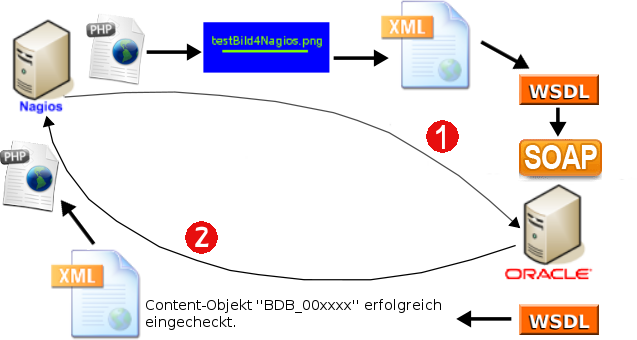
\includegraphics[width=0.93\textwidth]{bilder/wsdl.png}}
		\caption{Ablauf der Benutzersimulation}
		\label{usersim}
\end{figure}

\begin{figure}[ht]
	\centering
	   \fbox{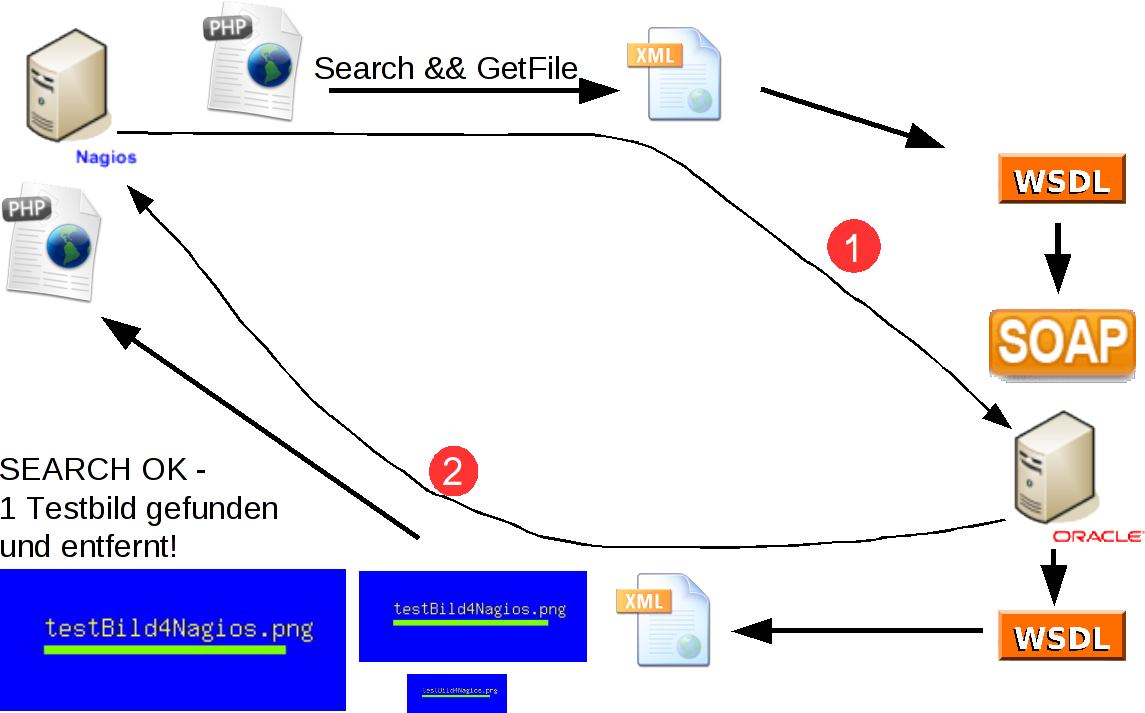
\includegraphics[width=0.93\textwidth]{bilder/wsdl-valid.png}}
		\caption{Überprüfung der Benutzersimulation}
		\label{usersim2}
\end{figure}
%
\begin{figure}[ht]
	\centering
	   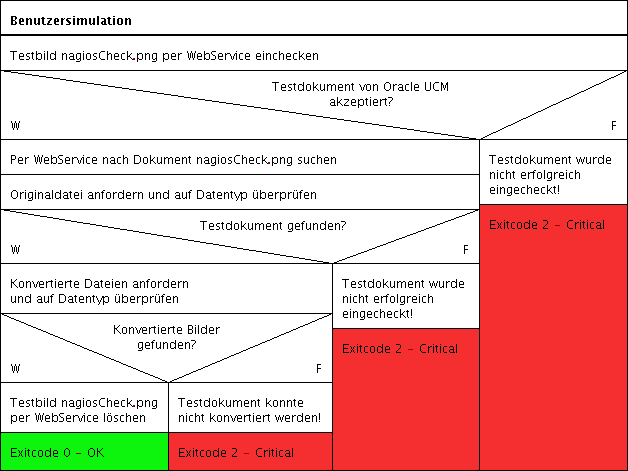
\includegraphics[width=0.9\textwidth]{bilder/Benutzersimulation.png}
		\caption{Ablauf der Benutzersimulation}
		\label{user-sim}
\end{figure}



